\documentclass{chi2009}
\usepackage{times}
\usepackage{url}
\usepackage{graphics}
\usepackage{color}
\usepackage[pdftex]{hyperref}
\usepackage{xspace}

\usepackage{graphicx}


\newcommand*{\system}{OGEN\xspace}
\newcommand*{\papertitle}{\system: Visualizing Physical Query Execution in a Relational Big Data Management System}
\newcommand*{\graph}{Physical Query Plan\xspace}
\newcommand*{\fragment}{Fragment Execution\xspace}
\newcommand*{\network}{Worker Communication\xspace}
\newcommand*{\overall}{Fragment Overall\xspace}

\hypersetup{%
pdftitle={\papertitle},
pdfauthor={Umar Javed, Thierry Moreau, Dominik Moritz, Adriana Szekeres},
pdfkeywords={},
bookmarksnumbered,
pdfstartview={FitH},
colorlinks,
citecolor=black,
filecolor=black,
linkcolor=black,
urlcolor=black,
breaklinks=true,
}
\newcommand{\comment}[1]{}
\definecolor{Orange}{rgb}{1,0.5,0}
\newcommand{\todo}[1]{\textsf{\textbf{\textcolor{Orange}{[[#1]]}}}}

\pagenumbering{arabic}  % Arabic page numbers for submission.  Remove this line to eliminate page numbers for the camera ready copy

\begin{document}
% to make various LaTeX processors do the right thing with page size
\special{papersize=8.5in,11in}
\setlength{\paperheight}{11in}
\setlength{\paperwidth}{8.5in}
\setlength{\pdfpageheight}{\paperheight}
\setlength{\pdfpagewidth}{\paperwidth}

% use this command to override the default ACM copyright statement
% (e.g. for preprints). Remove for camera ready copy.
%\toappear{Submitted for review to CHI 2009.}
\toappear{}

\title{\papertitle}
\numberofauthors{1}
\author{\alignauthor Umar Javed, Thierry Moreau, Dominik Moritz, Adriana Szekeres \\
\affaddr{Dept. of Computer Science, University of Washington} \\ \affaddr{ Seattle, Washington, USA} \\
\email{\texttt{\{ujaved, moreau, domoritz, aaasz\}@cs.washington.edu}}
}

\maketitle

\begin{abstract}

We propose a visualization system for understanding and exploring query execution and data movement in a distributed database management system (DDBMS). Our tool provides insight into: (1) data flow between query fragments and between workers, (2) query execution and operator dependencies, (3) cluster utilization, (4) network utilization. Our tool, which we call \system, helps developers understand and improve query execution, and provides insight into common problems such as data skew or performance bottlenecks.

In particular, \system is built to inspect query execution in Myria\footnote{\url{http://myria.cs.washington.edu/}}, a distributed big data management system currently being developed in the UW CSE database group. Myria aims towards building a distributed database platform to provide \emph{big data management and analytics as a service} primarily for scientific applications.

The proposed visualizations can easily be applied to other DDBMS as well (e.g. Spark, Hadoop).

\end{abstract}

%\keywords{put author keywords here}

%\category{H.5.2}{Information Interfaces and Presentation}{Miscellaneous}[Optional sub-category]

\section{Introduction}

% Umar

% What is myria, how does it work (look at report from last quarter but shorter), which languages are supported
% motivation
% questions (inspiration: https://docs.google.com/a/uw.edu/document/d/1Syn65bu_p6S4RQETaozsleYcRBauQJ7IduYrctS1wrw/edit?pli=1#)
% why is a visualization a good way to answer the questions

\begin{itemize}
    \item problem: hard to learn why a query is slow
    \item motivation: help developers/programmers dig what the problems might be
\end{itemize}


\section{Related Work}

Twitter developed Ambrose\cite{ambrose}, a platform for visualization and real-time monitoring of MapReduce data workflows. They offer three different views to show associated jobs, job dependencies and progress. Ambrose has been released as open source. Ambrose, however, is not suitable for our needs as the abstraction level of jobs is too high and does not capture single operators.

Google's Dapper\cite{sigelman2010dapper} is a distributed systems tracing infrastructure and offers fine grained tracing of calls in Google's distributed systems. They also proposed an interface for visualizing traces. Similarly, X-trace\cite{fonseca2007x} was developed as a framework to trace which events cause what other events in a distributed environment. recently, there has been work on visualizing event traces collected in X-trace\footnote{\url{https://github.com/brownsys/X-Trace/tree/master/src/webui/html/interactive}}. Due to the importance of these kinds of debug facilities, Twitter closely modeled Zipkin\cite{zipkin} after Dapper and X-trace and released it as open source.

Dapper and X-trace focus on how data flows through a distributed system. In \system the visualization focuses on the operators and how the data flows through them. This orthogonal view is better suited for debugging performance bottlenecks in DDBMS and also scales to a larger number of events. Furthermore, in contrast to  we offer different abstraction levels, which enables users to find problems faster and handle larger amounts of profiling data. Also, \system is specifically designed to help developers understand query execution in distributed database system like Myria as opposed to general traces in distributed systems.

Tools to visualize query plans for example in SQL Server, as used to improve performance for the SDSS Sky survey\cite{szalay2002sdss}, focus on optimizing queries and not query execution and have no visualization of data flow, which is necessary to optimize physical query execution.

\section{Approach}
\label{sec:approach}

% Adriana

The first step in designing \system was to identify the possible causes that
could affect the execution performance of the query. After we identified
several such causes, that we will enumerate below, we leveraged visualization
techniques that we found fit to allow developers/programmers to get insight
into how the query was executed on the available resources and quickly
identify the source(s) of the performance penalty.

We found that the performance of the query might be affected by the following
factors, which greatly influenced the design of our visualization tool:
\begin{itemize}
   \item \emph{Wrong/unoptimized physical query plan.} We manually analyzed
several physical query plans and discovered that some queries were poorly
optimized. This led us to design a view that allows interactive exploration of
the physical query plan (mapped to a graph of query operators). 
   \item \emph{Stragglers, tail latency, expensive query operators, poor
scheduling.} Our targeted systems are \emph{distributed} databases. Therefore,
as the query is executed in a distributed environment, the query coordinator
has to wait until all the workers finish executing their assigned tasks. To
give insight into how the tasks are distributed and executed at each workers,
we designed a view that shows the cluster utilization over time and at each
worker.
   \item \emph{Poor data partitioning, data skew.} Network traffic can cause
serious delay when executing a distributed query. Due to poor data
partitioning, workers might need to send unnecessary big amount of data between
each other. We designed a view that allows the developer/programmer to analyze
the data traffic generated while executing the query.  
\end{itemize} 

% Why did we choose the visualization
% How it is implemented
% explain how events and logs are used to create the raw data for vis

\system's architecture (Fig.~\ref{fig:arch}) consists of a back-end,
used as a plug-in interface for the distributed database system targeted, and a
front-end which implements the views described above. The front-end and
back-end of \system are highly decoupled so that the visualization can be used not only with
Myria but also with other systems such as Spark or Hadoop. In
Section~\ref{sec:back} we illustrate how we implemented log collections and
aggregation in Myria.

\subsection{Back-end}
\label{sec:back}

The task of the back-end is to log when operators are called, when the call returns and when data is sent to another worker. Using this data and simple transformations, we can obtain the information necessary to create the visualizations to answer the questions in Section~\ref{sec:approach}.

There are two possible approaches that we explored to collect event logs that can be used to extract spans and other performance related data necessary for the visualization. First, events could be logged to files using a standard logging tool and then collect the files on one node using remote copy. Once the logs are on one machine, the logs can be parsed and the data can be transformed into the desired format.

We switched to a different approach as shown in Figure~\ref{fig:arch} where logs are written directly into the worker's database. When the front-end requests the data, the master executes a query that collects the data and streams the results directly to the requesting client. Logs are thus tuples in a relation and no longer separate in files and in a custom format. Despite being more reliable, faster and using the same logic that Myria already implements, we are able to write queries to aggregate, filter and transform the collected data.

For example, the data for how many workers are working on a certain fragment as described in Section~\ref{sec:fragments} is generated from the event log using a query to select only events for the root operators (the operators that have no parent in the same fragment) in each fragment and a custom map function that carries state. The state is an integer that is incremented when the operator is called on a worker and decremented when the operator returns.

\begin{figure}[ht]
  \includegraphics[width=\columnwidth]{images/viz_arch}
  \caption{Overview of the log collection and transformation architecture. Raw event logs are collected on each worker. The data is stored in relations. To download the data, a query has to be executed.}
  \label{fig:arch}
\end{figure}

We highly suggest that developers use the second approach when porting \system to a new DDBMS.

\subsection{Front-end}

The Myria web front-end server is written in Python and runs on Google App Engine. \system's user-interface (UI) is embedded into Myria's web front-end. We build \system's UI using D3\cite{2011-d3} to deliver an interactive visualization experience to the user. D3 is a JavaScript framework for data visualziation on the web. We used visualization techniques such as \emph{focus+context}\cite{furnas1986generalized} that possible to implement conveniently using D3.

\system's front-end gets data from the Myria server as JSON and CSV files. JSON objects are used to describe the physical queryplan. CSV files contain logs on query execution at the fragment and operator level as well as data exchange between workers at different stages of the query execution.

\system's web UI is divided into two components: (1) the context window which provides a visualization of the \graph, and (2) the performance window which provides some insight into an element selected in the context view. The context window contains a view of the \graph, rendered as a graph. The user can navigate the \graph by expanding query fragments into the operators that compose it. The user can chose to select a fragment of interest which will render a \fragment visualization for the selected fragment in the performance window. Alternatively, the user can select an fragment-to-fragment edge in the \graph thus rendering a \network visualization for the selected edge in the performance window. If no elements are selected in the \graph view, an \overall visualization is rendered in the performance window, displaying the aggregate worker utilization over time for each fragment.

The following subsections describe each one of the four views offered by \system's web UI.

% Thierry

\subsubsection{Overview over all fragments}
\label{sec:fragments}

% Adriana

% Write about small multiples view

\subsubsection{Physical query plan view}

% Thierry

\subsubsection{Fragment execution view}

% Adriana

The \fragment view comprises two charts: the utilization chart and the
operators chart. The utilization chart (Fig.~\ref{fig:utilization_chart}) shows the utilization
of the cluster over time, inside the selected fragment. The chart is used to
quickly reveal any patterns in the schedule, like tail latency, long periods of
idleness, etc. We implemented a small brush (at the top of the figure) that
allows the user to zoom-in and further analyze the problematic area.

\begin{figure}[ht]
  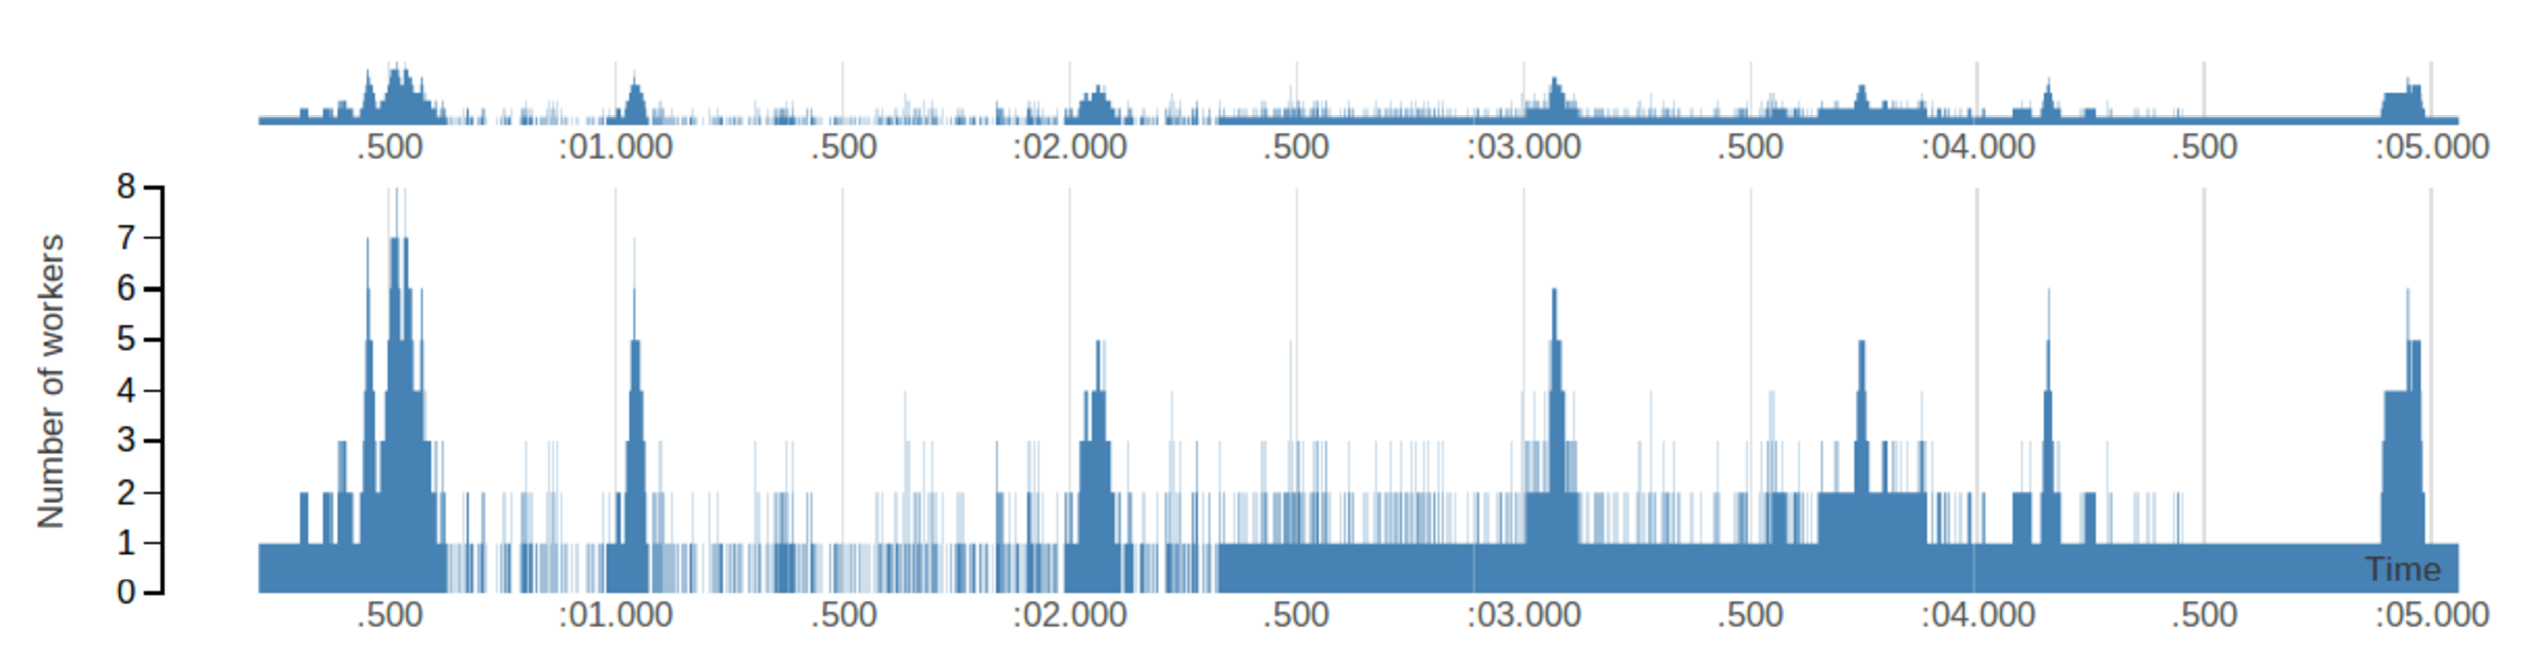
\includegraphics[width=\columnwidth]{images/utilization_chart}
  \caption{The utilization chart. }
  \label{fig:utilization_chart}
\end{figure}
  
The utilization chart also implements a brush that allows the user to further
analyze the query execution by displaying the schedule of each of the worker
nodes, in the operators chart (Fig.~\ref{fig:operators_chart}). The per-worker
schedule shows what operators the worker executed and for how long.


\begin{figure}[ht]
  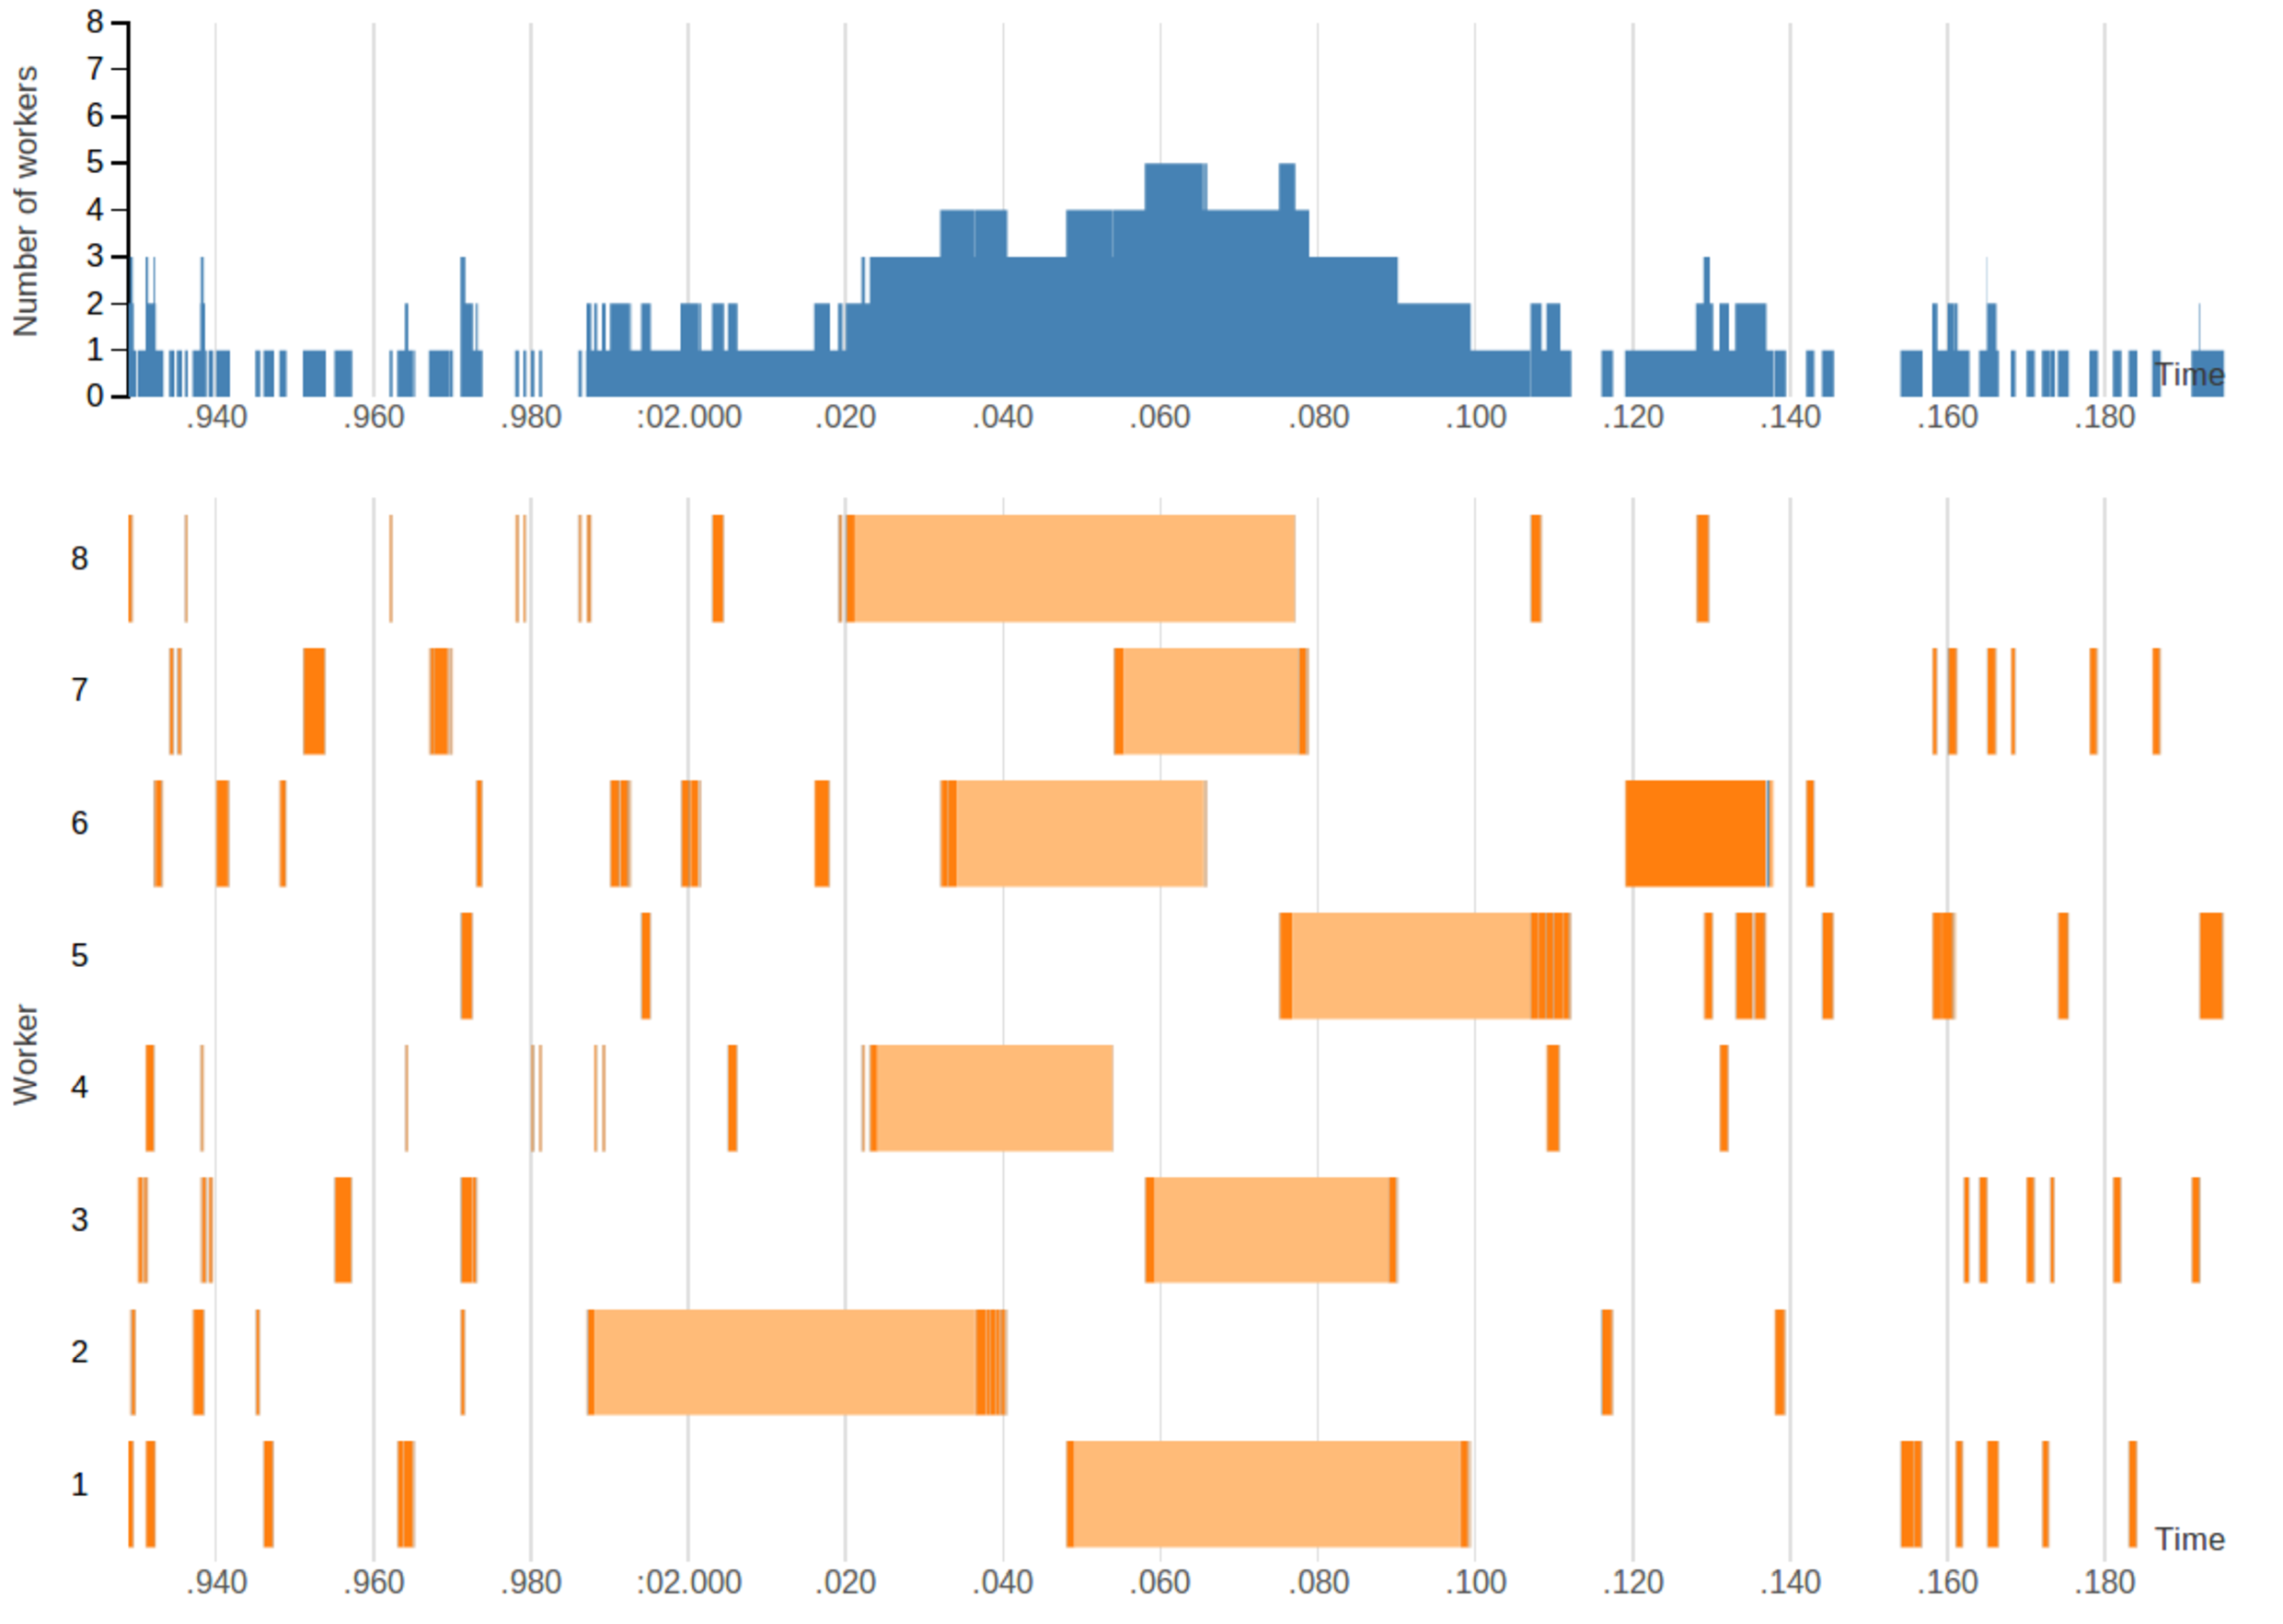
\includegraphics[width=\columnwidth]{images/operators_chart}
  \caption{The operators chart.}
  \label{fig:operators_chart}
\end{figure}

% use the word spans when referring to events with duration (used in dapper)

\subsubsection{Worker communication view}

% Umar

\section{Evaluation}

% How it helps
% Examples

% Thierry + Dom

\textbf{Discussion:}

\section{Conclusion}

% Adriana

\section{Future Work}

A focus of the current implementation is on scalability to many workers and long running queries. More aggregations have to be done by the database itself. Most importantly, in the fragment visualization that shows spans for all events we should limit the data that is being downloaded and rendered to what the user can see. With the architecture as explained in Section~\ref{sec:back}, we are able to express these filter conditions as queries.

Besides performance improvements, we plan to integrate X-trace and its visualization to offer the orthogonal view and allow users to trace how tuple batches flow through the operators and between operators. Combined with the visualizations described in this paper, it will form a powerful debugging tool that will help us to better understand and improve query execution.

\bibliographystyle{abbrv}
\bibliography{paper}

\end{document}
